%Optionally in the drone
\newpage
\subsection{Total Dissolved Solids}
Total dissolved solids (TDS) can be defined as the mass of residue remaining when a measured volume of filtered water is evaporated. TDS is usually written in ppm (parts per million).

While turbidity is about particles that are not dissolved in water, total dissolved solids are about particles that are totally dissolved in water. TDS is usually low for freshwater sources, at less than 500 ppm. Seawater contains about 500-30,000 ppm, while brackish water contains 30–40,000 ppm.

\begin{figure}[h]
\centering
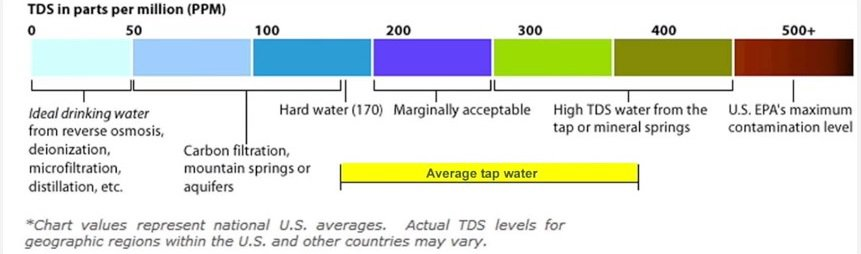
\includegraphics[scale=0.69]{water/91_tdschart.jpg}
\caption{TDS Chart for drinking water\cite{tdschart}}
\end{figure}

%Difference between conductivity sensor and tds sensor


\subsubsection{Sensors}
TDS sensors generally require temperature compensation in order to give accurate readings. Lower end models also generally require calibration from first use using a buffer solution of a known parts per million substance. \cite{sen0244wiki}

\paragraph{DFRobot SEN0244}\mbox{€11,66} \cite{SEN0244}
\begin{table}[h!]
	\centering
	\adjustimage{height=4cm,valign=c}{water/92_sen0244.jpg}\quad
	\begin{tabular}{| l | l |}
    \hline
    Protocol & Analog\\
    Operating Range & 0 ~ 1000ppm\\
    Measurement Accuracy &  100ppm \\
    Response time & Unknown \\
    Supply Voltage & 3.3V-5V \\
    Software library included & yes \\
    Availability & 3-5 Days \\
    \hline
	\end{tabular}
\end{table}
